%!TEX program = xelatex
% not lualatex because of a pgf bug: https://sourceforge.net/p/pgf/bugs/384/
\PassOptionsToPackage{table,svgnames}{xcolor}
\documentclass[11pt, book, english, french, standardlists]{upmethodology-document}
%!TEX root = ./RAPPORT_A17_INFO_ST40_PINARD_MAXIME.tex

% Encoding
	%\usepackage[utf8]{inputenc}
	%\usepackage[latin1]{inputenc}
	\usepackage[T1]{fontenc}

% Language
	%\usepackage[francais,english]{babel} % Second language = main language
	\usepackage[french]{translator}

% Show a summary of the layout of the current document with \layout.
	%\usepackage{layout}

% For easy management of document margins and the document page size.
	%\usepackage[top=2cm, bottom=1.8cm, left=1.8cm, right=1.8cm, head=14pt, foot=36pt]{geometry}

% Lets you change line spacing.
	%\usepackage{setspace}

% Euro symbol
	%\usepackage{eurosym}

% Fonts (include only one)
	%\usepackage{bookman}
	%\usepackage{charter}
	%\usepackage{newcent}
	\usepackage{lmodern}
	%\usepackage{mathpazo}
	%\usepackage{mathptmx}

% Enables typesetting of hyperlinks
	%\usepackage{url}
	\usepackage{hyperref}

% Verbatim environment
	%\usepackage{verbatim}
	%\usepackage{moreverb}
	\usepackage{fancyvrb}

% Code listing
	\usepackage{listings}

% To change header and footer of any page of the document.
	%\usepackage{fancyhdr}

% Allows you to insert graphic files within a document.
	%\usepackage{graphicx}

% Allows figures or tables to have text wrapped around them.
	%\usepackage{wrapfig}

% Adds support for colored text.
	\usepackage{xcolor}

% Allows tables rows and columns to be colored, and even individual cells.
	%\usepackage{colortbl}

% Mathematics
	\usepackage{amsmath}
	\usepackage{amssymb}
	\usepackage{mathrsfs}
	%\usepackage{asmthm}
	%\usepackage{mathtools}
	%\usepackage{bm} % Greek letters in math mode

% Provide the array and tabular environments
	\usepackage{array}

% Provide the tabularx environment
	\usepackage{tabularx}

% Provide the multirow command
	\usepackage{multirow}

% Provides control over the layout of the three basic list environments: enumerate, itemize and description.
	%\usepackage{enumitem}

% Interface to sectioning commands for selection from various title styles
	%\usepackage[nobottomtitles]{titlesec}

% Highly customized stacking of objects, insets, baseline changes, etc.
	\usepackage{stackengine}

% Routines for constrained scaling and stretching of objects, relative to a reference object or in absolute terms
	\usepackage{scalerel}

% Provides control over the typography of the Table of Contents, List of Figures and List of Tables, and the ability to create new ‘List of ...’.
	%\usepackage{tocloft}
	%\usepackage{titletoc}

% Advanced bibliography handling.
	%\usepackage{bibtex}
	%\usepackage{biblatex}

% Allows customization of appearance and placement of captions for figures, tables, etc.
	\usepackage[justification=centering]{caption}

% Provides the multicols environment which typesets text into multiple columns.
	%\usepackage{multicol}

% This package simplifies the insertion of external multi-page PDF or PS documents.
	%\usepackage{pdfpages}

% Prints out all index entries in the left margin of the text.
	%\usepackage{showidx}

% Allow to define multiple floats (figures, tables) within one environment giving individual captions and labels in the form 1a, 1b.
	%\usepackage{subcaption}

% Lets you insert notes of stuff to do with the syntax \todo{Add details.}.
	%\usepackage{todonotes}

% Text Companion fonts, which provide many text symbols (such as baht, bullet, copyright, musicalnote, onequarter, section, and yen), in the TS1 encoding.
	%\usepackage{textcomp}

% Supply landscape environment
	\usepackage{pdflscape}

% Floating elements placement
	\usepackage{float}

% Add document elements like a bibliography or an index to the Table of Contents.
	\usepackage[notindex,nottoc,notlot,notlof]{tocbibind}

% Allow TeX pictures or other TeX code to be compiled standalone or as part of a main document
	%\usepackage[subpreambles=true]{standalone}
	\usepackage{standalone}
	\usepackage{import}

% PGF-TikZ
	\usepackage{pgf}
	\usepackage{tikz}
	\usepackage{pgf-umlsd}
	\usepackage{pgfgantt}

% Change the typesetting of footnotes
	\usepackage[perpage,bottom]{footmisc}

% Defines commands \counterwithin and \counterwithout
	\usepackage{chngcntr}

% Allow creation of glossaries
	\usepackage[acronym,toc]{glossaries}

% Personnal packages
	\usepackage{packages/MagicListings}

%!TEX root = ./RAPPORT_A17_INFO_ST40_PINARD_MAXIME.tex

%----------------------------------------
% Figures configuration
%----------------------------------------

\usetikzlibrary{shapes}
\usetikzlibrary{arrows.meta}
\usetikzlibrary{calc}

\definecolor{bg_color}{RGB}{250,250,229}

\colorlet{color1}{cyan!50}
\colorlet{color2}{red!30!green!40}
\colorlet{color3}{orange!50}
\colorlet{color4}{violet!60!blue!55}

\newganttlinktype{bartobardown}{
	\ganttsetstartanchor{south east}
	\ganttsetendanchor{north west}
	\draw [/pgfgantt/link] (\xLeft, \yUpper) -- (\xRight, \yLower);
}
\newganttlinktype{bartobarup}{
	\ganttsetstartanchor{north east}
	\ganttsetendanchor{south west}
	\draw [/pgfgantt/link] (\xLeft, \yUpper) -- (\xRight, \yLower);
}
\newganttlinktype{milestonetobardown}{
	\ganttsetstartanchor{south}
	\ganttsetendanchor{north west}
	\draw [/pgfgantt/link] (\xLeft, \yUpper) -- (\xRight, \yLower);
}
\newganttlinktype{bartomilestonedown}{
	\ganttsetstartanchor{south east}
	\ganttsetendanchor{north}
	\draw [/pgfgantt/link] (\xLeft, \yUpper) -- (\xRight, \yLower);
}


%----------------------------------------
% upmethodology commands redefinition
%----------------------------------------

\makeatletter

% Remove 'Initials' column from validators
\renewcommand{\upm@document@addvalidator}[3][]{%
	\global\protected@edef\thevalidatorlist{\thevalidatorlist\protect\Ifnotempty{\thevalidatorlist}{,} \protect\upmmakename{#2}{#3}{~}}

	\global\protected@edef\upm@document@validator@tab@commented{\upm@document@validator@tab@commented \protect\upmmakename{#2}{#3}{~} & 
	& \protect\Ifnotempty{#1}{\protect\href{mailto:#1}{#1}}\\}

	\ifupm@document@validator@tab@hascomment\else
		\global\protected@edef\upm@document@validator@tab{\upm@document@validator@tab \protect\upmmakename{#2}{#3}{~} & 
		\protect\Ifnotempty{#1}{\protect\href{mailto:#1}{#1}}\\}
	\fi
}
\renewcommand{\upm@document@addvalidatorstar}[4][]{%
	\global\protected@edef\thevalidatorlist{\thevalidatorlist\protect\Ifnotempty{\thevalidatorlist}{,} \protect\upmmakename{#2}{#3}{~}}

	\global\let\upm@document@validator@tab\relax

	\global\protected@edef\upm@document@validator@tab@commented{\upm@document@validator@tab@commented \protect\upmmakename{#2}{#3}{~} & 
	#4 & \protect\Ifnotempty{#1}{\protect\href{mailto:#1}{#1}}\\}

	\upm@document@validator@tab@hascommenttrue
}
\renewcommand{\upmdocumentvalidators}[1][\linewidth]{%
	\ifupm@document@validator@tab@hascomment%
		\Ifnotempty{\upm@document@validator@tab@commented}{%
		\noindent\expandafter\begin{mtabular}[#1]{3}{|X|l|c|}%
		\tabulartitle{\upm@lang@document@validators}%
		\tabularheader{\upm@lang@document@names}{\upm@lang@document@comments}{\upm@lang@document@emails}%
		\upm@document@validator@tab@commented
		\hline%
		\expandafter\end{mtabular}\par\vspace{.5cm}}%
	\else%
		\Ifnotempty{\upm@document@validator@tab}{%
		\noindent\expandafter\begin{mtabular}[#1]{2}{|X|c|}%
		\tabulartitle{\upm@lang@document@validators}%
		\tabularheader{\upm@lang@document@names}{\upm@lang@document@emails}%
		\upm@document@validator@tab
		\hline%
		\expandafter\end{mtabular}\par\vspace{.5cm}}%
	\fi%
}

% Remove history from document info page
\renewcommand{\upmdocinfopage}{
	\thispagestyle{plain}
	\upmdocumentsummary\upmdocumentauthors\upmdocumentvalidators\upmdocumentinformedpeople\clearpage%
}

% Decrease space after upmcaution upminfo and upmquestion message boxes
\renewenvironment{upm@highligh@box}[2]{%
	\par
	\vspace{.5cm}
	\begin{tabular}{|p{#1}|}
	\hline
	\begin{window}[0,l,{\mbox{\includegraphics[width=1cm]{#2}}},{}]
}{%
	\end{window}\\ \hline \end{tabular}
	%\vspace{.5cm}
	\par
}

\makeatother

%----------------------------------------
% upmethodology informations
%----------------------------------------

% Document Information and Declaration
\declaredocument{Rapport de stage ST40 - A2017}{Développement et fiabilisation d’un module de désassemblage interne}{-}

% Document Authors
\addauthor*[maxime.pinard@utbm.fr]{Maxime}{Pinard}{Étudiant en branche INFO}

% Document Validators
\addvalidator*[jean-charles.creput@utbm.fr]{Jean-Charles}{Creput}{Suiveur UTBM}
\addvalidator*[benoit.amiaux@intradef.gouv.fr]{Benoît}{Amiaux}{Tuteur en entreprise}

% Informed People
\addinformed*[jean-charles.creput@utbm.fr]{Jean-Charles}{Creput}{Suiveur UTBM}
\addinformed*[benoit.amiaux@intradef.gouv.fr]{Benoît}{Amiaux}{Tuteur en entreprise}
\addinformed*[laure.foissard@intradef.gouv.fr]{Laure}{Foissard}{Responsable administratif (DRH)}

% Copyright and Publication Information
\setcopyrighter{Maxime Pinard}
\setpublisher{l'Universitée de Technologie de Belfort Montbéliard}

% Version
\incversion{\makedate{\the\day}{\the\month}{\the\year}}{Version initiale.}{\upmpublic}

%----------------------------------------
% utbmcovers informations
%----------------------------------------

\UseExtension{utbmcovers}

\setutbmfrontillustration{cover}
\setutbmtitle{Développement et fiabilisation d’un module de désassemblage interne}
\setutbmsubtitle{Rapport de stage ST40 - A2017}
\setutbmstudent{Maxime Pinard}
\setutbmstudentdepartment{Département Informatique}
\setutbmstudentpathway{}
\setutbmcompany{Direction générale de l'armement\\Maîtrise de l’information}
\setutbmcompanyaddress{Route de Laillé\\ 35131 Bruz, France}
\setutbmcompanywebsite{\href{http://www.defense.gouv.fr/dga}{\color{utbm_cover_main_shadow_text}{http://www.defense.gouv.fr/dga}}}
\setutbmcompanytutor{Benoît Amiaux}
\setutbmschooltutor{Jean-Charles Creput}
\setutbmkeywords{
	% Branche d'activité économique
	Armement \textendash{}
	SSII, services informatiques \textendash{}
	% Métiers
	Informatique \textendash{}
	Etude, développement \textendash{}
	% Domaine technologique
	Génie logiciel \textendash{}
	Sécurité \textendash{}
	% Application physique directe
	Logiciel d'analyse de données \textendash{}
	Analyse de binaires
}
\setutbmabstract{
	La Direction Générale de l'Armement (DGA) est une direction du Ministère des Armées qui a de nombreuses missions dont celle de préparer l'avenir des systèmes de défense français, pour cela plusieurs centres d'expertise et d'essais sont répartis en France tels que la DGA Maîtrise de l'Information (DGA MI) situé près de Rennes. La DGA MI a pour mission des études, expertises et essais dans les domaines de la guerre électronique, des systèmes d'armes, des systèmes d'information, des télécommunications, de la sécurité de l'information et des composants électroniques.
	\vspace{12pt}\\
	Au sein de la DGA MI des équipes travaillent sur l’analyse de binaires dont le code source est inconnu, pour cela deux types d'analyses sont utilisées, l'analyse dynamique en suivant l'exécution du programme à l'aide d'un débogueur et l'analyse statique en étudiant le code désassemblé sans exécuter le programme.
	\vspace{12pt}\\
	GenDbg est un débogueur générique développé en interne de la DGA MI, conçu pour pouvoir déboguer tout type de programme, il repose sur de nombreux modules spécifiques aux caractéristiques du programme débogué. Le module de désassemblage pour les architectures de processeurs MIPS de GenDbg étant obsolète et non maintenu, ma première mission a été de réaliser une nouvelle implémentation de ce dernier en utilisant la librairie de désassemblage Capstone.
	\vspace{12pt}\\
	Hex-Rays IDA est un logiciel d'analyse statique qui permet de documenter un binaire pour en comprendre le fonctionnement, la DGA MI développe et maintient un plugin IDA nommé YaCo qui permet de travailler à plusieurs sur une même base de code. YaCo, initialement codé en Python, a été porté en C++, la deuxième mission de mon stage a été de réaliser le portage C++ et l'amélioration des parties responsables de la gestion du dépôt Git et des événements IDA.
}

%----------------------------------------
% Listings
%----------------------------------------

\lstalias[gendbg]{C}[GenDbg]{C}
\lstdefinelanguage[gendbg]{C}{
	language={[StandardLibrary]C},
	morekeywords=[1]{
		__cdecl
	},
	morekeywords=[2]{
		DWORD
	},
	morekeywords=[2]{
		AsmBankInfo_T,
		AsmAddressSpaceInfo_T,
		AsmAddressTypeInfo_T,
		AsmGroupRegisterInfo_T,
		AsmDataInfo_T,
		AsmDecodedInstruction_T,
		AsmInstructionInfo_T,
		AsmModuleInfo_T,
		CPUCtx_T,
		GenDbgHelperAsmInfo_T,
		MemoryAddress_T,
		MemoryArea_T,
		ViewCtx_T,
		AsmModuleFnIdx_T,
		MIPS_RegisterId_T
	},
	morekeywords=[2]{
		cs_insn,
		cs_detail,
		cs_x86,
		cs_arm64,
		cs_arm,
		cs_m68k,
		cs_mips,
		cs_ppc,
		cs_sparc,
		cs_sysz,
		cs_xcore,
		cs_tms320c64x,
		cs_mips_op,
		mips_reg,
		mips_op_mem
	},
	morekeywords=[3]{
		CS_MNEMONIC_SIZE
	}
}

\lstalias[yaco]{C}[YaCo]{C}
\lstdefinelanguage[yaco]{C}{
	language={[StandardLibrary]C},
	morekeywords=[1]{
		__cdecl
	},
	morekeywords=[2]{
		ssize_t,
		hook_type_t,
		hook_cb_t
	},
	morekeywords=[3]{
		idaman,
		ida_export,
		idaapi,
		HT_IDP,
		HT_UI,
		HT_DBG,
		HT_IDB,
		HT_DEV,
		HT_VIEW,
		HT_OUTPUT,
		HT_GRAPH,
		HT_LAST
	}
}


%----------------------------------------
% Other configurations
%----------------------------------------

% Figures folder
\graphicspath{{figures/}}

% Figures counting
\counterwithout{figure}{chapter}

% Table counting
\counterwithout{table}{chapter}

% Source code formatting
\upmcodelang{cpp}

% Prevent page breaks in paragraphs
\predisplaypenalty=1000
\postdisplaypenalty=1000
\clubpenalty=1000

% Minimal space required in the bottom margin not to move the title on the next page
%\renewcommand{\bottomtitlespace}{.1\textheight}

% Links config, especialy for the table of contents
\hypersetup{
    colorlinks=true,
    linkcolor=black,
    urlcolor=blue,
    linktoc=all
}

% French language config
\frenchbsetup{StandardLayout=true,ReduceListSpacing=false,CompactItemize=false}

% Vertical alignement config
\raggedbottom{}

\setglossarystyle{list}

%----------------------------------------
% Functions definitions
%----------------------------------------

% Clear to the next left page
\newcommand*{\cleartoleftpage}{
  \clearpage \ifodd\value{page}\hbox{}\newpage\fi
}

% Paragraph with line break
\newcommand{\p}[1]{\paragraph{#1\\}}

% Function to print a warning sign
\newcommand{\dangersign}[1][2.5ex]
	{\renewcommand{\stacktype}{L}
		{\scaleto{\stackon[1pt]{\color{red}$\triangle$}{\fontsize{4pt}{4pt}\selectfont !}}{#1}}}

% Definition of \Witem for 'itemize' environment with a warning sign
\newcommand{\Witem}
{\item[\dangersign{}]}

\newcommand{\annexe}[1]{Annexe \ref{sec:#1}}
\newcommand{\file}[1]{\texttt{#1}}
\newcommand{\folder}[1]{\texttt{#1}}
\newcommand{\reg}[1]{\texttt{\$#1}}


\makeglossaries
%!TEX root = ./RAPPORT_A17_INFO_ST40_PINARD_MAXIME.tex

\newacronym{API}{API}{Application programming interface}
\newacronym{ASC}{ASC}{Architecture de systèmes C3R}
\newacronym{C3R}{C3R}{Commandement, communication, conduite et renseignement}
\newacronym{CASSI}{CASSI}{Centre de l'armement pour la SSI}
\newacronym{CCSA}{CCSA}{Centre de calculs scientifique de l'armement}
\newacronym{CEA}{CEA}{Commissariat à l'énergie atomique et aux énergies alternatives}
\newacronym{CELAR}{CELAR}{Centre d’électronique de l'armement}
\newacronym{CGN}{CGN}{Capteur guidage navigation}
\newacronym{COMM}{COMM}{Département central d’information et de communication}
\newacronym{DATAR}{DATAR}{Délégation à l'aménagement du territoire et à l'action régionale}
\newacronym{DCN}{DCN}{Direction des constructions navales}
\newacronym{DGA MI}{DGA MI}{DGA maîtrise de l'information}
\newacronym{DGA-old}{DGA}{Délégation Générale pour l'Armement}
\newacronym{DGA}{DGA}{Direction générale de l'armement}
\newacronym{DGRIS}{DGRIS}{Direction générale des relations internationales et de la stratégie}
\newacronym{DGSE}{DGSE}{Direction générale de la sécurité extérieure}
\newacronym{DGSIC}{DGSIC}{Direction générale des systèmes d’information et de communication}
\newacronym{DICoD}{DICoD}{Délégation à l’information et à la communication de la défense}
\newacronym{DIRISI}{DIRISI}{Direction interarmées des réseaux d’infrastructure et des systèmes d’information de la défense}
\newacronym{DI}{DI}{Direction du développement international}
\newacronym{DLL}{DLL}{Dynamic Link Library}
\newacronym{DMA}{DMA}{Délégation ministérielle pour l'armement}
\newacronym{DO}{DO}{Direction des opérations}
\newacronym{DPID}{DPID}{Direction de la protection des installations, moyens et activités de la défense}
\newacronym{DP}{DP}{Direction des Plans, des Programmes, et du Budget}
\newacronym{DRH}{DRH}{Direction des ressources humaines}
\newacronym{DRM}{DRM}{Direction du renseignement militaire}
\newacronym{DRSD}{DRSD}{Direction du renseignement et de la sécurité de la défense}
\newacronym{DS}{DS}{Direction de la stratégie}
\newacronym{DT}{DT}{Direction technique}
\newacronym{EMA}{EMA}{État-major des armées}
\newacronym{ETPT}{ETPT}{équivalent temps plein travaillé}
\newacronym{FPU}{FPU}{Floating point unit}
\newacronym{GArm}{GArm}{Gendarmerie de l’armement}
\newacronym{GIAT}{GIAT}{Groupement industriel des armements terrestres}
\newacronym{GPR}{GPR}{General Purpose Register}
\newacronym{GTest}{GTest}{Google Test}
\newacronym{GTE}{GTE}{Geometry transformation engine}
\newacronym{GUI}{GUI}{Graphical user interface}
\newacronym{HTTP}{HTTP}{Hypertext transfer protocol}
\newacronym{ISA}{ISA}{Instruction set architecture}
\newacronym{MC}{MC}{Matériaux composants}
\newacronym{MIPS}{MIPS}{Microprocessor without interlocked pipeline stages}
\newacronym{MRIS}{MRIS}{Mission pour la recherche et l’innovation scientifique}
\newacronym{OIAS}{OIAS}{Organisation interarmées du soutien}
\newacronym{OTAN}{OTAN}{Organisation du traité de l'Atlantique nord}
\newacronym{PPC}{PPC}{PowerPC}
\newacronym{RISC}{RISC}{Reduced instruction set computer}
\newacronym{SCA}{SCA}{Service du commissariat des armées}
\newacronym{SCSSI}{SCSSI}{Service central de la sécurité des systèmes d'informations}
\newacronym{SDS}{SDS}{Système de systèmes}
\newacronym{SEA}{SEA}{Service des essences des armées}
\newacronym{SGA}{SGA}{Secrétariat général pour l’administration}
\newacronym{SIAé}{SIAé}{Service industriel aéronautique}
\newacronym{SIMu}{SIMu}{Service interarmées des munitions}
\newacronym{SMA}{SMA}{Service de la maintenance aéronautique}
\newacronym{SMQ}{SMQ}{Service central de la modernisation et de la qualité}
\newacronym{SM}{SM}{Soutien métrologie}
\newacronym{SPR}{SPR}{Special Purpose Register}
\newacronym{SSA}{SSA}{Service de santé des armées}
\newacronym{SSDI}{SSDI}{Service de la sécurité de défense et de l’information}
\newacronym{SSF}{SSF}{Service de soutien de la flotte}
\newacronym{SSI}{SSI}{Sécurité des systèmes d'informations}
\newacronym{SSTIC}{SSTIC}{Symposium sur la sécurité des technologies de l'information et des communications}
\newacronym{UE}{UE}{Union européenne}
\newacronym{UTBM}{UTBM}{Université de technologie de Belfort Montbéliard}
\newacronym{VIM/VSE}{VIM/VSE}{Rétro-ingénierie et analyse de malwares et produits logiciels}

\begin{document}
	\chapter*{Remerciements}
		\paragraph*{}
			Je tiens tout particulièrement à remercier mon maître de stage \textbf{Benoît Amiaux} pour m'avoir permis de travailler sur des sujets intéressants et formateurs. Je le remercie aussi pour le suivi et les conseils qu'il m'a apportés au cours du stage, ainsi que pour l'indépendance et la confiance qu'il m'a accordée.
		\paragraph*{}
			Ensuite, je tiens à remercier \textbf{les membres l'équipe VIM/VSE} pour leur accueil chaleureux, pour toutes les informations et les conseils qu'ils m'ont donnés ainsi que pour leur bonne humeur aux différentes pauses-café et repas.
		\paragraph*{}
			Je remercie aussi \textbf{la direction de la DGA} pour m'avoir permis de  joindre leur personnel durant ces quelques mois ainsi que \textbf{Laure Foissard} du Bureau de Gestion des Emplois et Compétences de la DGA et \textbf{Mireille Jacquot} du Service des Stages de l'UTBM pour la gestion de mon dossier.
	\tableofcontents{}
	\listoffigures{}
	\chaptertoc{Introduction}
		\paragraph*{}
			Le cursus à l'\gls{UTBM} est entrecoupé de deux périodes de stage de 6 mois durant les 3 ans du cycle ingénieur, après le Tronc Commun. La première, après un an en branche, est le ST40 intitulé ``Stage Assistant Ingénieur'' et la seconde, un an plus tard, est le ST50 intitulé ``Projet de fin d'études - Ingénieur débutant''.
		\begin{figure}[H]
			\centering%
			\resizebox{\textwidth}{!}{\import{figures/}{Cursus_INFO_UTBM.tex}}%
			\caption{Cursus en informatique a l'\acrshort{UTBM}}%
			\label{fig:Cursus_INFO_UTBM}%
		\end{figure}
		\paragraph*{}
			Ce rapport concerne mon ST40 que j'ai réalisé à la \gls{DGA} Maîtrise de l'Information sur le site de Bruz, près de Renne du 1er Aout 2017 au 26 Janvier 2018 sous la supervision de mon maitre de stage, Benoît Amiaux.
		\paragraph*{}
			La \gls{DGA} est une direction du Ministère des Armées qui a de nombreuses missions dont celle de préparer l'avenir des systèmes de défense français, en particulier sur le plan informatique avec son centre d'expertise et d'essais Maîtrise de l'Information. De ce fait, la \gls{DGA MI} est un acteur français important de la sécurité informatique. Ce dernier proposant un sujet intéressant qui correspondait à mes compétences, j'ai donc saisi l'opportunité d'y réalisé mon stage.
		\paragraph*{}
			Le sujet du stage implique de nombreux concepts bas niveau, ce qui m'intéresse particulièrement et m'a en partie poussé à choisir ce sujet, préférant travailler plus proche de la machine.  Le sujet est le développement et la fiabilisation d'un module de désassemblage \acrshort{MIPS} pour un débugger développé en interne. Le développement du module est en C/C++ et implique l'assemblage et le désassemblage de code, la gestion des adresses\ldots. Ainsi le sujet a l'avantage d'allier des concepts très bas niveau avec un développement dans des langages plus haut niveau.
		\paragraph*{}
			Je commencerai par présenter le Ministère des armées, la \gls{DGA} et la \gls{DGA MI}, j'expliciterai ensuite le sujet et l'organisation du stage avant de détailler le déroulement de ce dernier. Par la suite sera développé le travail réalisé sur le sujet initial ainsi que sur le sujet additionnel, ajouté au cours du stage.
	\chapter{Présentation de l'entreprise}
		\section{Le Ministère des Armées}
			\begin{upminfo}
				Nommé ``Ministère des Armées'' au début de la 5e république, il devient ``Ministère de la Défense nationale'' en 1969 puis ``Ministère de la Défense'' en 1974 avant de reprendre le nom de ``Ministère des Armées'' en 2017. Il est donc normal qu'il soit désigné par ``Ministère de la Défense'' dans les documents (Code de la défense, décrets\ldots) datant d'avant 2017.
			\end{upminfo}
			\subsection{Responsabilités}
				\paragraph*{}
					<<Le ministre de la défense est responsable de la préparation et de la mise en œuvre de la politique de défense. Il est en particulier chargé de l'infrastructure militaire comme de l'organisation, de la gestion, de la mise en condition d'emploi et de la mobilisation des forces armées et des formations rattachées[\ldots].
				\paragraph*{}
					Il a autorité sur les armées, les services de soutien, les organismes interarmées et les formations rattachées. Il veille à ce que ceux-ci disposent des moyens nécessaires à leur entretien, leur équipement et leur entraînement. Il est responsable de leur sécurité.
				\paragraph*{}
					Il est également chargé:
					\begin{itemize}
						\item de la prospective de défense;
						\item du renseignement extérieur et du renseignement d'intérêt militaire;
						\item de l'anticipation et du suivi des crises intéressant la défense;
						\item de la politique industrielle et de recherche et de la politique sociale propres au secteur de la défense.>>\cite{CodeDefenseL1142-1}
					\end{itemize}
			\subsection{Composition}
				\paragraph*{}
					<<L'administration centrale du ministère de la défense est composée:
					\begin{enumerate}
						\item De l'état-major des armées;
						\item Des organismes militaires et des services interarmées rattachés au chef d'état-major des armées;
						\item Des états-majors de l'armée de terre, de la marine et de l'armée de l'air;
						\item De la direction générale de l'armement;
						\item Du secrétariat général pour l'administration;
						\item De directions générales, directions et services.>>\cite{DEFD0918712D}
					\end{enumerate}
			\subsection{Budget}
				\paragraph*{}
					Le budget du Ministère de la défense vient de 3 crédits qui sont répartis sur trois missions:
					\begin{itemize}
						\item Défense
						\item Anciens combattants, mémoire et liens avec la Nation
						\item Recherche et enseignement supérieur au titre du programme Recherche duale
					\end{itemize}
				\paragraph*{}
					En 2017 le budget total est de 43,2 milliards d'euros, soit 13,6\% (10,2\% hors pensions) du budget total de l'État (détaillé sur la figure \ref{fig:Budget_Ministere_Defense_2017}). Dans le respect de la Loi de programmation militaire 2014-2019, de son actualisation en 2015 et des décisions prises à la suite des attentats de 2015 et de 2016, le budget de la mission ``Défense'' a été augmenté de 700 millions d'euros de 2015 à 2016 et de 600 millions d'euros de 2016 à 2017, le portant ainsi à 32,7 milliards d'euros.
				\begin{figure}[H]
					\centering%
					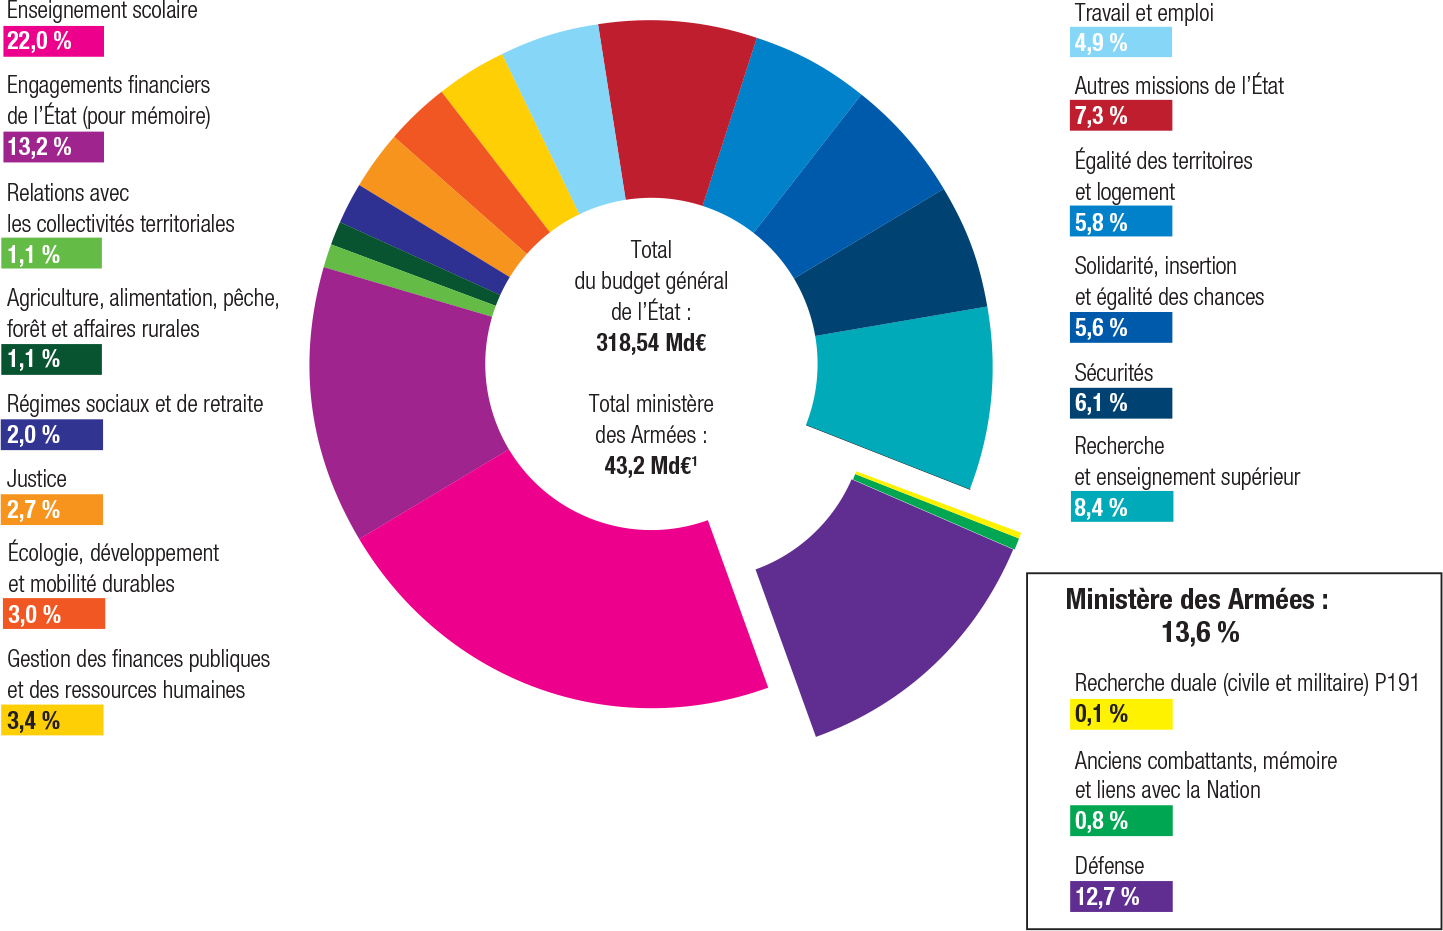
\includegraphics[width=1\textwidth]{Budget_Ministere_Defense_2017}
					\caption{Part du budget du Ministère de la Défense (pensions incluses) dans le budget général de l'État en 2017\cite{ChiffresDef2017}}%
					\label{fig:Budget_Ministere_Defense_2017}%
				\end{figure}
			\subsection{Effectifs}
				\paragraph*{}
					En 2016 le Ministère de la défense avait un effectif total de 265 458 \gls{ETPT}, composé à 77\% de militaires et 23\% de civils (voir détails sur la figure \ref{fig:Effectifs_Ministere_Defense_2016}). L'age moyen du personnel militaire était de 33,2 ans et celui du personnel civil de 47,4 ans.
				\begin{figure}[H]
					\centering%
					\resizebox{0.8\textwidth}{!}{\import{figures/}{Effectifs_Ministere_Defense_2016.tex}}%
					\caption*{\small\itshape Autres services = \acrshort{SCA}, \acrshort{SSA}, \acrshort{DGA}, \acrshort{SGA} (dont \acrshort{DICoD}), \acrshort{DIRISI}, \acrshort{SEA}, \acrshort{SIMu}, \acrshort{OIAS}, \acrshort{DRM}, \acrshort{DRSD}, \acrshort{DGSE}, \acrshort{DPID}, \acrshort{DGSIC}, \acrshort{DGRIS} et \acrshort{EMA} (partie centrale)}%
					\caption{Répartition des effectifs du Ministère de la Défense en 2016, par gestionnaire, en \acrshort{ETPT}\cite{ChiffresDef2017}}%
					\label{fig:Effectifs_Ministere_Defense_2016}%
				\end{figure}
		\section{La Direction générale de l'Armement}
			\subsection{Historique}
				\paragraph*{}
					En 1961, le général de Gaulle crée la \gls{DMA} pour rationaliser la construction des matériels militaires, elle compte 6 corps d'ingénieur militaires\footnote{Les ingénieurs militaires sont des experts techniques au service de la défense}: les ingénieurs de l'aéronautique, les ingénieurs militaires des fabrications d'armement, les ingénieurs du génie maritime, les ingénieurs hydrographes de la marine, les ingénieurs des poudres et les ingénieurs militaires des télécommunications. En 1968, ils sont remplacés par un corps unique: le corps des ingénieurs de l'armement. En 1977, la \acrshort{DGA-old} signifiant alors ``Délégation Générale pour l'Armement'' est créée pour remplacer la \gls{DMA}.
				\paragraph*{}
					En 1995, l'arrivée de Jean-Yves Helmer au poste de délégué général pour l'armement\footnote{Jean-Yves Helmer sera a la tête de la \acrshort{DGA-old} de 1996 à 2001} lancera un mouvement de regroupement et d'externalisation de la production industrielle. Regroupement d'une part par la fusion des implantations territoriales pour former 14 grands centres ainsi que la réduction du personnel qui passera de plus de 50 000 en 1995 à 9 700 en 2017. D'autre part externalisation car la \acrshort{DGA-old} passe d'une structure de production d'armement à une agence de maîtrise d'ouvrages complexes. Ainsi, la \acrshort{DGA-old} se séparera graduellement de ses activités industrielles.
					% \begin{itemize}
					% 	\item[1990] Le \gls{GIAT} de la \gls{DGA} devient la société anonyme \gls{GIAT} Industries (aujourd'hui Nexter System, détenu par l'État français)
					% 	\item[1991] La \gls{DCN} devient une société de droit privé à capitaux publics sous le nom de DCNS (aujourd'hui Naval Group, détenu à 62,49\% par l'État français)
					% 	\item[2000] Le \gls{SSF} est créé pour assurer dans une structure unique la maîtrise d'ouvrage de la mise en condition opérationnelle des bâtiments de surface et des sous-marins de la Marine nationale
					% 	\item[2007] Le \gls{SMA} est transféré à l'état-major de l'armée de l'air et renommé \gls{SIAé}
					% 	\item[2010] Le Centre d'Études de Gramat, responsable de l'évaluation des vulnérabilités des systèmes d'armes aux agressions des armes nucléaires et conventionnelles, est transféré au \gls{CEA}
					% \end{itemize}
				\paragraph*{}
					Le 5 octobre 2009, le décret n°2009-1180\cite{DEFD0918712D} officialise le changement de nom et d'organisation de la ``Délégation Générale pour l'Armement'' qui devient dès lors ``Direction Générale de l'Armement'', toujours abrégé \gls{DGA}.
			\subsection{Missions}
				\paragraph*{}
					La \gls{DGA} est une direction du Ministère des Armées, elle dépend non pas du Chef d'État-Major des Armées mais directement du ministre de la Défense. Elle a de très nombreuses missions (listées dans le décret n°2009-1180\cite{DEFD0918712D}, Article 1) dont on peut extraire trois missions principales:
				\p{Équiper les forces armées}
					Maître d'ouvrage des programmes d'armement, la \gls{DGA} est responsable de la conception, de l'acquisition et de l'évaluation des systèmes qui équipent les forces armées. Son action couvre toute la durée de vie de ces programmes.
				\p{Préparer l'avenir}
					Imaginer les futurs possibles, anticiper les menaces et les risques, préparer les capacités technologiques et industrielles, dans un cadre européen.
				\p{Promouvoir les exportations d'armement}
					Contribuer activement aux exportations d'armement tant sur l'aspect contrôle pour le respect des engagements internationaux de la France que sur l'aspect économique pour le développement des entreprises de défense.
			\subsection{Organisation}
				\paragraph*{}
					Depuis le 9 août 2017, Joël Barre est Délégué Général pour l'Armement (voir organigramme en \annexe{organigrammedga}), ce dernier, pour mener a bien les missions de la \gls{DGA}, s'appuie sur différents services (dont les attributions exactes sont détaillées dans le décret n°2009-1180\cite{DEFD0918712D}), organisés la plupart du temps sous forme matricielle:
				\p{Direction du Développement International} % décret n°2009-1180\cite{DEFD0918712D}, Article 6
					La \gls{DI} est chargée de la promotion des exportations d'armement en s'appuyant notamment sur le réseau des attachés d'armement. Elle anime et coordonne le soutien de l'État aux industriels exportateurs, en liaison étroite avec les états-majors et le réseau diplomatique.
				\p{Direction des opérations} % décret n°2009-1180\cite{DEFD0918712D}, Article 4
					La \gls{DO}\footnote{anciennement Direction des systèmes d'armes} est chargée de la conduite des programmes et opérations d'armement, et est chargée de l'exécution des travaux d'études en amont. La \gls{DO} est chargée de l'acquisition des systèmes d'armes, équipements de défense, matériels et logiciels en liaison avec les états-majors, et en assurant la cohérence entre les programmes.
				\p{Direction de la Stratégie} % décret n°2009-1180\cite{DEFD0918712D}, Article 5
					La \gls{DS}, à Bagneux, est en charge de la stratégie pour la recherche technologique, l'industrie, et les programmes d'armement menés en coopération en s'appuyant notamment sur la \gls{MRIS}.
				\p{Direction des Plans, des Programmes, et du Budget} % décret n°2009-1180\cite{DEFD0918712D}, Article 8
					La \acrlong{DP} (\acrshort{DP}\footnote{anciennement DPBG}) est chargée de la planification, de la programmation, de la préparation et de l'exécution du budget et assure la maîtrise financière et comptable des opérations d'armement conduites par la \gls{DGA}.
				\p{Services de soutien} % décret n°2009-1180\cite{DEFD0918712D}
					Le \gls{SMQ}, l'inspection, le \gls{COMM}, le \gls{SSDI}, la \gls{DRH}, la \gls{GArm}.
				\p{Direction Technique} % décret n°2009-1180\cite{DEFD0918712D}, Article 7
					La \gls{DT} assure les activités d'essai et d'expertise des matériels et des technologies militaires à l'aide de différents pôles de compétences. De nombreux centres d'expertise et d'essais interviennent dans le test des technologies de pointe, ces derniers sont dispersés sur toute la France (voir la figure \ref{fig:Carte_centres_expertise_et_essais_DGA}).
					\begin{figure}[H]
						\centering
						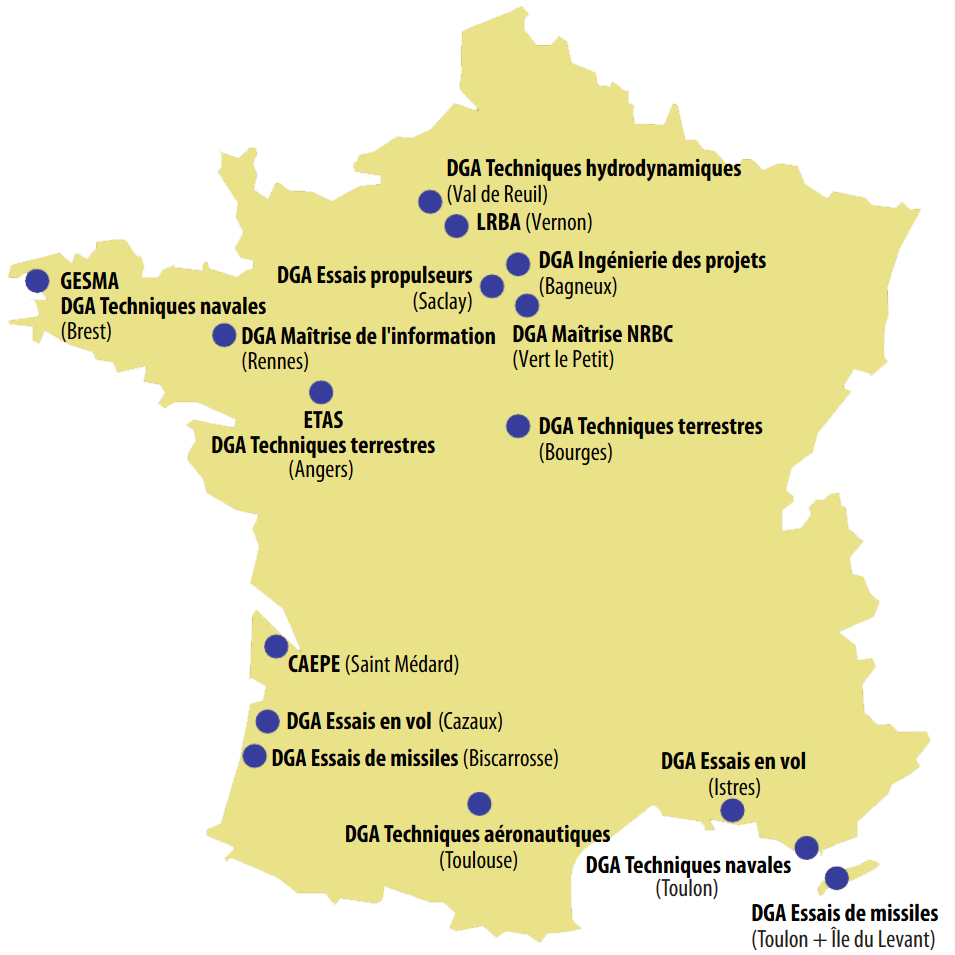
\includegraphics[width=0.9\textwidth]{Carte_centres_expertise_et_essais_DGA}
						\caption{Carte des centres d'expertise et d'essais de la \acrshort{DGA}\cite{OptroDefDGA}}
						\label{fig:Carte_centres_expertise_et_essais_DGA}
					\end{figure}
			\subsection{Effectifs et budget}
				\paragraph*{}
					En 2017 la \gls{DGA} a un effectif de 9 700 personnes dont plus de 51\% d'ingénieurs et cadres\cite{PresentationDGA}. Bien que membre à part entière du ministère de la Défense, la \gls{DGA} se distingue par une forte proportion de civils au sein de son personnel, 55,7\% pour la \gls{DGA} contre une moyenne de 22,9\% pour le Ministère de la Défense dans son ensemble en 2015\cite{ChiffresDef2016}, mais aussi par la quasi-absence de sous-officiers, aucun pour la \gls{DGA} contre une moyenne de 44,9\% pour le Ministère de la Défense dans son ensemble en 2016\cite{ChiffresDef2017}.
				\paragraph*{}
					Le budget de la \gls{DGA} n'est pas public, mais représente une part conséquente du budget du Ministère de la défense pour pouvoir maintenir, en 2017, 80 programmes d'armement et maintenir sa position de premier investisseur public de France, avec près de 11 milliards d'euros de commandes passées pour la seule année 2017. De plus la \gls{DGA} maintient une présence internationale dans 20 pays, y compris auprès de l'\gls{OTAN} et de l'\gls{UE}\cite{PresentationDGA}.
		\section{La DGA Maîtrise de l'Information}
			\subsection{Historique}
				\paragraph*{1961}
					<<Un conseil interministériel présidé par Georges Pompidou décide de favoriser le développement de l'économie de la Bretagne en y encourageant l'implantation de l'industrie électronique. Au détriment du choix initial de Grenoble, Rennes doit devenir le second pôle de l'électronique en France derrière Paris.>>\cite{CELAR40ansAvenir}
				\paragraph*{1964}
					% L'ingénieur militaire en chef de 1ère classe des télécommunications Émile Rombout est chargé de diriger les opérations de création du centre.
					La décision est prise de créer le \gls{CELAR}. <<Le cahier des charges précise que le terrain aura une superficie de 15 à 30 hectares, à 15 km de Rennes maximum. Il bénéficiera de vues dégagées, sera éloigné de sources de perturbations radioélectriques et sera attractif comme un terrain déjà planté en arbres tel un parc à l'instar des autres centres d'études et de recherche récemment implantés.>>\cite{CELAR40ansAvenir}
				\paragraph*{1966}
					Début de construction du \gls{CELAR} sur un terrain de 108 hectares situé à Bruz. <<Le coût total de l'opération est estimé à 41 millions de francs dont 25 millions à la charge de la \gls{DATAR} et 16 millions à celle du ministère des Armées>>\cite{CELAR40ansAvenir}
				\paragraph*{1968}
					Ouverture du \gls{CELAR}, les deux premières années l'activité technique du \gls{CELAR} consiste essentiellement en des travaux de simulation et d'évaluation de matériels.
				\paragraph*{1970-1980}
					Le \gls{CELAR} étend ses activités, accueille le \gls{CCSA} et développe ses capacités de conseil. Le \gls{CELAR} investit dans le domaine la guerre électronique et des systèmes spatiaux.
				\paragraph*{1980-1990}
					Les simulations numériques et hybrides prennent leur essor. L'analyse technologique des composants électroniques se renforce. En 1986, est instauré le \gls{SCSSI}\cite{DecretCreationSCSSI} dont la conséquence sera la scission de la \gls{SSI} en France entre le secteur commercial prit en charge par le Ministère des Télécommunications et le secteur gouvernemental prit en charge par le Ministère de la Défense. Les premières actions relevant de la \gls{SSI} au \gls{CELAR} sont des travaux dans le domaine des évaluations des produits de chiffrement gouvernementaux.
				\paragraph*{1990-2000}
					À l'issue de la guerre du Golfe, le \gls{CELAR} est désigné comme le centre technique de la \gls{DGA} pour la guerre électronique. Il développe ses compétences pour la sécurité des systèmes d'information. En 1993, \gls{CCSA} disparaît pour laisser place au \gls{CASSI}. <<L'approche est singulière dans le contexte du moment qui jusque-là a une tendance lourde a repousser vers le secteur privé toutes les activités alors industrielles de l'État. Pour la \gls{SSI}, il s'agit en effet de rapatrier en sphère étatique les activités alors industrielles de production des algorithmes cryptographiques gouvernementaux, de réalisation des composants cryptographiques et de définition des équipements de chiffrement.>>\cite{CELAR40ansAvenir} % Toujours en 1993, une première machine est installée sur le réseau internet, c'est une station SUN sous Unix.
				\paragraph*{2000-2010}
					Le \gls{CELAR} devient le centre de référence européen des techniques de la guerre de l'information, dans un contexte des systèmes pour une sécurité globale. Les effectifs \gls{SSI} se multiplient face au besoin de sécurisation de tous les ministères. <<Par ailleurs, les systèmes d'armes font une entrée massive dans la zone d'action de la \gls{SSI}. [\ldots] Les torpilles, avions, chars et missiles sont désormais dotés de capacités de calcul, de stockage et d'échange d'informations, tout comme les machines informatiques classiques.>>\cite{CELAR40ansAvenir}\\
					En 2005 le \gls{CELAR} se réorganise en six divisions:
					\begin{itemize}
						\item \acrfull{CGN}
						\item \acrfull{SSI}
						\item \acrfull{MC}
						\item \acrlong{ASC}\footnote{Commandement, Communication, Conduite et Renseignement} (\acrshort{ASC})
						\item \acrfull{SDS}
						\item \acrfull{SM}
					\end{itemize}
					En 2009 le \gls{CELAR} est renommé en \acrfull{DGA MI}, son patrimoine brut est alors évalué à plus de 323 millions d'euros.
				\p{2010-2018}
				\noindent\vspace{-7mm}
					\begin{upmcaution}
						Au sein de la \gls{DGA} et de nombreux projets classé secrets se déroulent sur plus de 10 ans, il n'est donc pas possible de diffuser des informations relatives à l'évolution de la \gls{DGA MI} sur ces dernières années.
					\end{upmcaution}
			\subsection{Missions}
				\paragraph*{}
					La \gls{DGA MI} est un centre d'expertise technique de la \gls{DGA} qui a pour mission:
					\begin{itemize}
						\item L'aide à la spécification d'architecture de systèmes et ingénierie des systèmes
						\item Expertise et évaluation de l'utilisation du spectre des fréquences
						\item Expertise des réseaux de télécommunication et des systèmes de transmission
						\item Spécification, évaluation et validation de l'interopérabilité des systèmes de commandement et de communication
						\item Spécification et évaluation des systèmes de renseignement (capteurs spatiaux, drones\ldots)
						\item Évaluation de la sécurité des systèmes d'information, conception et évaluation de produits de sécurité
						\item Évaluation des performances de systèmes d'armes, de guerre électronique et de guerre optronique
						\item Expertise des systèmes de missiles tactiques et stratégiques
						\item Expertise de composants électroniques spécifiques pour la défense
					\end{itemize}
			\subsection{Organisation}
				\begin{upminfo}
					L'organisation de la \gls{DGA MI} est Diffusion Restreinte, c'est-à-dire qu'elle n'est pas classée secrète mais qu'elle porte une mention particulière de confidentialité, tout élément d'organisation ne concernant pas le stage ne sera donc pas abordé.
				\end{upminfo}
				\paragraph*{}
					Pour mon stage, j'ai rejoint les départements \gls{VIM/VSE} au sein de la division \gls{SSI}5. Les départements \gls{VIM/VSE} ont été créés en 2017, les deux équipes se connaissant bien et partageant le même étage ainsi que la même salle de pause, j'ai donc autant côtoyé la partie VIM que VSE.
				\begin{figure}[H]
					\centering
					\resizebox{\textwidth}{!}{\import{figures/}{Hierarchie_DGA_MI_a_VIM.tex}}
					\caption{Hiérarchie de la \acrshort{DGA MI} à \acrshort{VIM/VSE}}
					\label{fig:Hierarchie_DGA_MI_a_VIM}
				\end{figure}
				\paragraph*{}
					Un schémas plus complet reprenant la hiérarchie des Ministères français à VIM/VSE est disponible en \annexe{hierarchieministereavim}.
		\section{Le secret}
			\subsection{Classification}
				\paragraph*{}
					<<Les informations et supports classifiés font l'objet d'une classification comprenant trois niveaux:
					\begin{enumerate}
						\item Très Secret-Défense;
						\item Secret-Défense;
						\item Confidentiel-Défense.>>\cite{CodeDefenseR2311-2}
					\end{enumerate}
				\paragraph*{}
					<<Le niveau Très Secret-Défense est réservé aux informations et supports qui concernent les priorités gouvernementales en matière de défense et de sécurité nationale et dont la divulgation est de nature à nuire très gravement à la défense nationale.
				\paragraph*{}
					Le niveau Secret-Défense est réservé aux informations et supports dont la divulgation est de nature à nuire gravement à la défense nationale.
				\paragraph*{}
					Le niveau Confidentiel-Défense est réservé aux informations et supports dont la divulgation est de nature à nuire à la défense nationale ou pourrait conduire à la découverte d'un secret de la défense nationale classifié au niveau Très Secret-Défense ou Secret-Défense.>>\cite{CodeDefenseR2311-3}
				\paragraph*{}
					Les documents qui ont fait l'objet de mesures de classification au niveaux cité précédemment relèvent de l'article 413-9 du Code Pénal\cite{CodePenal413-9}.
				\paragraph*{}
					<<Nul n'est qualifié pour connaître des informations et supports classifiés s'il n'a fait au préalable l'objet d'une décision d'habilitation et s'il n'a besoin, selon l'appréciation de l'autorité d'emploi sous laquelle il est placé, au regard notamment du catalogue des emplois justifiant une habilitation établi par cette autorité, de les connaître pour l'exercice de sa fonction ou l'accomplissement de sa mission.>>\cite{CodeDefenseR2311-7}
			\subsection{Diffusion Restreinte}
				\paragraph*{}
					<<Certaines informations qu'il n'y a pas lieu de classifier peuvent cependant recevoir, de la part de leur émetteur, une marque de confidentialité destinée à restreindre leur diffusion à un domaine spécifique [\ldots] ou à garantir leur protection (telle que Diffusion Restreinte).
				\paragraph*{}
					Ces mentions, qui ne traduisent pas une classification, ne suffisent pas à conférer aux informations concernées la protection pénale propre au secret de la défense nationale. Leur seul objectif est de sensibiliser l'utilisateur à la nécessaire discrétion dont il doit faire preuve dans la manipulation des informations couvertes par cette mention.
				\paragraph*{}
					L'auteur de la divulgation, qu'il relève de la sphère publique ou de la sphère privée, s'expose à des sanctions disciplinaires ou professionnelles, sans préjudice de l'application éventuelle des dispositions spécifiques au traitement et à la protection de données à caractère personnel.
				\paragraph*{}
					La mention Diffusion Restreinte [\ldots] indique que l'information ne doit pas être rendue publique et ne doit être communiquée qu'aux personnes ayant besoin de la connaître dans l'exercice de leurs attributions.>>\cite{PRMD1132480A}
			\subsection{Application au stage}
				\paragraph*{}
					Les projets des départements \gls{VIM/VSE} sont souvent classifiés au niveau Confidentiel-Défense. Cela implique donc des règles de sécurité très strictes et un cloisonnement des projets. Toujours pour des raisons de sécurité, les règles de sécurité, moyens de cryptage utilisés, vérification des données et autres systèmes de sécurité mis en place ne pourront pas être détaillés dans ce rapport.
				\paragraph*{}
					La liste des membres des équipes, l'organigramme de la division ou encore activités exactes menées sont soit Diffusion Restreinte soit classé secrètes. Cependant les travaux réalisés par \gls{VIM/VSE} impliquent souvent l'analyse de binaires dont le code source est inconnu, pour cela des outils externes tel que IDA de Hex-Rays sont utilisés mais aussi des outils internes dont GenDbg, un débogueur générique et YaCo, un plugin qui permet le travail collaboratif avec IDA.
				\paragraph*{}
					Durant mon stage, j'ai justement travaillé sur ces outils internes (GenDbg et YaCo) dont les informations ne sont ni classées secrètes ni Diffusion Restreinte. GenDbg a été présenté publiquement au \gls{SSTIC} de 2008\cite{SSTICGenDbg} et YaCo à celui de 2017\cite{SSTICYaCo}. %Les membres de l'équipe travaillent sur différentes missions mais ont une partie de leur temps de travail dédié au développement des outils dont ils peuvent avoir besoin tels que GenDbg et YaCo.
	\chapter{Organisation du stage}
		\section{GenDbg}
			\subsection{Présentation}
				\paragraph*{}
					Il existe une multitude d'architectures matérielles et des langages et chaque environnement de développement logiciel intègre un outil de débogage plus ou moins évolué. De ce fait, les outils de débogage ne cessent de se multiplier. GenDbg est un débogueur développé et utilisé en interne à la \gls{DGA MI} depuis plus de 10 ans, il a pour but de proposer une solution générique, cohérente et évolutive à ce problème.
				\paragraph*{}
					Le projet présente trois grands avantages:
					\begin{itemize}
						\item \textbf{Maîtrise}: contrôle de tous les aspects du cycle de vie logiciel et indépendance vis-à-vis de tout éditeur de logiciels
						\item \textbf{Modularité}: constitué d'un cœur et d'une multitude de modules pour permettre un enrichissement fonctionnel très rapide et facilement paramétrable
						\item \textbf{Généricité}: certainement le principal intérêt du projet, il est possible d'exécuter pas-à-pas un programme quel que soit son mode d'exécution sur n'importe quelle plate-forme et n'importe quel système d'exploitation
					\end{itemize}
				\paragraph*{}
					GenDbg permet de déboguer tout type de programme (code machine, byte code java, P-Code visual basic, DotNet,\ldots) sur des architectures hétérogènes. Pour cela, il adopte un modèle framework / stub qui permet de séparer les composants débogués et la machine de l'analyste. En fonction du type d'analyse envisagé (malware) on préférera travailler sur deux machines physiques distinctes. Cette approche avec des stubs permet aussi de réduire l'empreinte du débogueur sur la cible. Le framework est capable de communiquer avec les stubs via un port série ou des canaux nommés (pipes).
				\paragraph*{}
					Les modules obligatoires au fonctionnement de GenDbg sont le stub, le framework, le module ASM (module de désassemblage) et le \gls{GUI}\footnote{interface graphique}. Historiquement seul un \gls{GUI} en ``mode texte'' était disponible mais une seconde interface, graphique cette fois, et réalisée avec Qt fut développé plus tard. Une vue de Gendbg utilisant le GUI Qt ainsi que sa lecture est présente en \annexe{guiqtgendbg} ainsi que la lecture de la vue Code en \annexe{guiqtgendbgvuecode}.
				\begin{figure}[H]
					\centering
					\resizebox{\textwidth}{!}{\import{figures/}{GenDbg_architecture_minimale.tex}}
					\caption{GenDbg: Architecture minimale}
					\label{fig:GenDbg_architecture_minimale}
				\end{figure}
				\paragraph*{}
					Concrètement, et en utilisant les notations de la figure \ref{fig:GenDbg_architecture_minimale}, pour exécuter un programme pas-à-pas avec GenDbg, il faut:
					\begin{itemize}
						\item Sur l'ordinateur 1:\\
							Exécuter le stub correspondant à l'architecture de l'ordinateur avec en paramètre le programme a analyser ainsi que le canal de communication a utiliser. Le stub se chargera de lancer l'application.
						\item Sur l'ordinateur 2:\\
							Spécifier le canal de communication à utiliser dans le fichier de configuration de GenDbg puis exécuter le framework. Le framework se chargera des récupérer les informations nécessaires du stub, tel que le module ASM a utiliser et chargera le \gls{GUI}, permettant d'exécuter l'application pas-à-pas.
					\end{itemize}
				\paragraph*{}
					L'ordinateur 1 pouvant être une machine différente de l'ordinateur 2, ou bien la même machine, ou encore une machine virtuelle.
			\subsection{Fonctionnement}
				\p{Le framework}
					C'est la partie centrale de GenDbg, c'est une application Win32 qui prend en charge la communication inter-modules, implémente le jeu de commandes de base commun à l'ensemble des modules ainsi que le moteur de script historique. Le moteur de script historique est maintenant très peu utilisé puisque des bindings Python sont  disponibles et utilisables dans une console Python intégré au \gls{GUI} Qt, permettant de scripter directement en Python dans GenDbg.
				\paragraph*{}
					<<Tous les modules sont implémentés sous forme de librairies dynamiques et sont chargés dans l'espace d'adressage du framework après identification de la cible par un stub.
				\paragraph*{}
					Le framework a en charge la lecture d'un fichier de configuration (.ini) pour tenter d'établir un canal de communication avec un stub et l'initialisation des différents modules. Dans l'état actuel du projet le framework est capable de communiquer avec les stubs via un port série ou des canaux nommés (pipes). Il est ainsi possible de déboguer aussi bien des machines physiques que des machines virtuelles (VMWare ou VirtualPC) en mappant un port série virtuel sur un canal nommé.
				\paragraph*{}
					Le framework fournit aux différents modules un jeu de fonctions de base qui vont permettre d'interagir entre eux.>>\cite{SSTICGenDbg}
				\p{Les stubs}
					<<Les stubs s'exécutent sur la machine cible et prennent en charge la gestion des exceptions sur l'architecture cible; à ce titre ils sont fortement dépendants de l'architecture et de l'OS de la cible. Les stubs fournissent les services de base au framework, c'est-à-dire les accès en lecture et en écriture aux registres et à la mémoire. Ils réalisent aussi l'identification précise de la cible pour le framework, l'identification conduisant au chargement des modules utiles et disponibles.>>\cite{SSTICGenDbg}
				\p{Les modules ASM}
					<<Les modules ASM sont en fait des dés-assembleurs/assembleurs prenant en charge la représentation du code, des données et des adresses propres à l'architecture cible. Par exemple sur l'architecture IA32, en mode virtuel protégé une adresse mémoire est de la forme ``\jcode{sélecteur:offset}'' avec le sélecteur sur 16 bits et l'offset sur 32 bits. C'est le module ASM IA32 qui a la charge de la représentation visuelle d'une adresse virtuelle.>>\cite{SSTICGenDbg}
				\p{Les modules additionnels}
					En plus des modules obligatoires, un certain nombre de modules spécifiques optionnels sont définis:
					\begin{itemize}
						\item \textbf{Les Command Modules}:\\
							Ils complètent les commandes de base implémentées dans le framework avec des commandes spécifiques au contexte d'exécution de la cible.
						\item \textbf{Les OS Helper Modules}:\\
							Ils offrent des services et des fonctionnalités propres à un système d'exploitation parmi lesquelles la signalisation d'un certain nombre d'événements internes.
						\item \textbf{Les Breakpoint Helpers Modules}:\\
							Ils permettent la prise en charge et la définition de points d'arrêt spécifiques à l'architecture cible.
						\item \textbf{Les Symbol Modules}:\\
							Ils permettent d'associer un symbole à une adresse particulière dans un module de l'OS cible.
					\end{itemize}
					Ces modules ne sont pas concernés par le stage et n'ont pas été utilisés, ils ne seront pas plus détaillés dans ce rapport.
				\p{Modularité et généricité}
					De par son architecture (représentée sur la figure \ref{fig:GenDbg_modules}) GenDbg déplace les spécificités hors du framework, les spécificités d'architecture et d'OS à déboguer se trouvent donc au niveau des stubs tandis que celles dues à la représentation (instructions, adresses\ldots) se trouvent au niveau des modules ASM. De même toutes les fonctionnalité spécifiques supplémentaires se trouvent au niveau des modules additionnels. Cela permet d'avoir un framework générique qui n'a pas besoin d'être modifié pour étendre les fonctionnalités de GenDbg. Cela permet aussi d'avoir un développement très ciblé, pour développer un nouveau module, il est seulement nécessaire de connaître l'\gls{API} que GenDbg expose aux modules et l'\gls{API} que le module expose à GenDbg.
				\p{Implémentation}
					Le framework est écrit en C, mais de par l'architecture modulaire, ne restreint pas le langage d'écriture des stubs et modules, le \gls{GUI} Qt est par exemple lui en C++. Dans les faits la plupart des stubs et modules sont, eux aussi, écrit en C. Certains stubs sont implémentés nativement d'autres le sont sous la forme de ``wrapper'' qui réalisent la traduction du protocole GenDbg vers le protocole d'un autre débogueur (par exemple gdb\footnote{Débogueur standard du projet GNU} et jdb\footnote{Débogueur Java de Oracle}).
				\begin{figure}[H]
					\centering
					\resizebox{\textwidth}{!}{\import{figures/}{GenDbg_modules.tex}}
					\caption{L'architecture modulaire du framework de GenDbg}
					\label{fig:GenDbg_modules}
				\end{figure}
			\subsection{Gestion du projet}
				\paragraph*{}
					Le projet n'étant pas une mission de la division mais un outil interne, son développement s'est étalé sur de nombreuses années et beaucoup de personnes ont travaillé dessus, souvent sur de courtes durées, sur les heures allouées au développement des outils internes.
				\paragraph*{}
					L'intégralité du code (framework, modules et stubs) est géré avec le gestionnaire de version Git, mais, pour des raisons de sécurité, il n'y a pas de serveur avec un repo synchronisé, ce dernier est passé par support physique entre les développeurs.
				\paragraph*{}
					La compilation est gérée avec CMake qui peut générer le projet pour différentes cibles (le plus souvent Visual Sudio) permettant de compiler le projet. Toutes les dépendances sont contenues dans le projet et compilées avec, à l'exception de Qt qui doit être installé sur la machine pour compiler le \gls{GUI} Qt.
				\paragraph*{}
					Il n'y a pas de normes de documentation, cette dernière est très peu présente en dehors des \gls{API} exposées par GenDbg et les modules. Il n'y avait, avant le stage, pas de tests, ceux que j'ai ajoutés sont gérés et exécutés avec CMake et utilisent la librairie \gls{GTest}.
			\subsection{Travail a réaliser}
				\paragraph*{}
					Le but initial du stage était le développement et la fiabilisation d'un module de désassemblage basé sur la librairie Capstone pour les architectures \acrshort{MIPS} et PowerPC. Le développement nécessitant d'implémenter toutes les fonctionnalités d'un module ASM GenDbg dont l'assemblage et le désassemblage en réalisant l'interfaçage entre GenDbg et Capstone. La fiabilisation elle, nécessitant la réalisation et la validation de tests unitaires sur les modules développés.
				\begin{figure}[H]
					\centering
					\resizebox{\textwidth}{!}{\import{figures/}{GenDbg_modules_impl.tex}}
					\caption{Implémentation des modules GenDbg et librairies utilisées}
					\label{fig:GenDbg_modules_impl}
				\end{figure}
				\paragraph*{}
					Lorsqu'il est évoqué d'utiliser la librairie Capstone, c'est en réalité la librairie Capstone et Keystone qui sont concernées, la première réalisant le désassemblage et la deuxième l'assemblage de code pour de nombreuses architectures, elles seront abordées plus en détail dans le chapitre \ref{ch:gendbg}. Certains modules utilisent déjà des librairies, c'est le cas des modules x86 et AMD64 qui utilisent déjà Capstone et Keystone. Les librairies étant déjà présentes, elles sont déjà intégrées au système de compilation, il suffira d'ajouter la liaison aux modules \acrshort{MIPS} et \acrshort{PPC} lors de leur compilation.
				\paragraph{}
					Le travail à réaliser est donc très technique et ne requiert pas d'étude préalable des cas d'utilisation ou d'identification des besoins, la conception du logiciel, son architecture et les différentes \gls{API} étant déjà présente et non modifiables au cours du stage. Il sera nécessaire d'étudier les différentes \gls{API} utilisables (GenDbg et Capstone) pour réalisé l'\gls{API} demandée (module ASM) tout en s'assurant de l'évolutivité du module.
				\paragraph*{}
					Le stage a commencé par la réalisation du module pour l'architecture \acrshort{MIPS} (détaillé au chapitre \ref{ch:gendbg}). À la fin de la réalisation de ce dernier cependant il fut décidé qu'il serait plus intéressant de ne pas réaliser le module pour l'architecture \acrshort{PPC}, pour à la place travailler sur le projet YaCo. %(présenté dans la section suivante et détaillé au chapitre \ref{ch:yaco}).
		\section{YaCo}
			\subsection{Présentation}
				TODO
			\subsection{Fonctionnement}
				TODO
			\subsection{Gestion du projet}
				TODO
			\subsection{Travail a réaliser}
				TODO
		\section{Déroulement du stage}
			\subsection{Conditions de travail}
				\p{Horaires}
					Mes horaires de travail pendant le stage étaient 8h30 -- 16h45, mais ces dernières n'étaient pas strictes et il m'était possible de rester plus tard pour compenser en cas de retard le matin ou simplement pour finir quelque chose avant de partir. La pause de midi était de 45 minutes et en général l'équipe se réunissait dans le couloir pour aller manger ensemble au restaurant d'entreprise.
				\p{Badge et zones}
					Le site de la \gls{DGA MI} est très sécurisé et un badge est nécessaire pour entrer et se déplacer sur le site, le badge donne accès au site, mais est aussi nécessaire pour accéder aux bureaux. J'ai obtenu mon badge assez tardivement (voir figure \ref{fig:Planning}), avant son obtention, j'avais un badge visiteur ne me permettant pas d'avoir accès à un bureau mais une solution temporaire a vite été trouvée et j'ai rapidement pu commencer à travailler.
				\p{Accès internet}
					Toujours dans un but de sécurité, les postes de travail ne sont reliés a aucun réseau afin de limiter leurs interactions avec des données étrangères. L'accès à internet se fait donc par un poste dédié qui est simplement une machine Windows avec uniquement un navigateur internet et un montage logiciel et réseau permettant de s'assurer de la sécurité de la connexion. Une fois le badge obtenu et un bureau attribué, j'ai été équipé d'un poste dédié pour accéder à internet.
				% \p{Logiciels}
				% 	Pour travailler sur GenDbg et YaCo, il m'était indispensable d'avoir CMake, git, Python, Hex-Rays IDA et un environnement de développement C/C++. J'ai travaillé durant la totalité du stage sous Windows 10 avec Microsoft Visual Studio 2017 et Sublime Text 3. En plus des logiciels indispensables cités avant j'ai aussi utilisé plusieurs outils de visualisation graphique pour Git. % + VirtualBox, QEMU Alpine Linux, Debian MIPS, TeXLive pour la présentation...
			\subsection{Planning}
				Voir figure \ref{fig:Planning}.
				\begin{landscape}
					\begin{figure}[H]
						\vspace*{-0.5cm}
						\hspace*{-2cm}
						\centering
						\resizebox{1.2\paperwidth}{!}{\import{figures/}{Planning.tex}}
						\caption{Planning}
						\label{fig:Planning}
					\end{figure}
				\end{landscape}
				\paragraph*{}
					Comme visible sur la figure \ref{fig:Planning}, j'ai commencé par le travail sur GenDbg avec le développement du module \acrshort{MIPS}, j'ai ensuite testé le module tout en effectuant les modifications et corrections nécessaires. Par la suite, à partir de mi Octobre, j'ai commencé à travailler sur YaCo en commençant par le Repository et en continuant sur les Hooks.
				\paragraph*{}
					Lors de mon travail plusieurs code review\footnote{revues de code} ont été réalisées par mon maître de stage, ce dernier m'indiquant des corrections et améliorations a réalisé dans mon code. Je suis donc parfois retourné travailler sur le travail précédant afin d'appliquer les modification demandées dans la revue de code.
				\paragraph*{}
					Enfin, le travail sur YaCo a donné lieu a deux pull request\cite{GithubYaCoPR24,GithubYaCoPR30} sur le repo publique du projet sur GitHub\cite{SSTICYaCo}.
				\paragraph*{}
					Après avoir terminé le travail sur GenDbg et YaCo, j'ai préparé une présentation orale interne a la \gls{DGA MI} sur le contenu de mon stage qui a eu lieu le 23 Janvier 2018. En parallèle à cela, j'ai commencé la rédaction du rapport de stage que j'ai continué sur les 3 jours restants après la présentation.
	\chapter{GenDbg}\label{ch:gendbg}
		\section{L'architecture MIPS}
			\subsection{Présentation}
				TODO
			\subsection{Particularités}
				TODO
			\subsection{Backward-compatibilité}
				TODO
			\subsection{Coprocesseurs}
				TODO
			\subsection{Documentation}
				TODO
		\section{Compilation}
			\subsection{Le système en place}
				\paragraph*{}
					CMake est une famille d'outils multiplateformes et open-source conçus pour compiler, tester et déployer des logiciels. CMake est utilisé pour contrôler la compilation d'un logiciel en utilisant des fichiers de configuration indépendants de la plate-forme et du compilateur à partir desquels seront générés des makefiles et projets pour de nombreux IDE et compilateurs.
				\paragraph*{}
					Le système de compilation et de tests de GenDbg utilise CMake pour ne dépendre d'aucune plateforme ou compilateur particulier, pour cela un fichier (\file{CMakeLists.txt}) définit plusieurs cibles pour CMake. Chaque cible correspond a un ou plusieurs fichiers de sortie (\acrshort{DLL}, exécutable\ldots). Les principales cibles sont:
					\begin{itemize}
						\item Le framework (\file{GenDbg.exe}), c'est l'exécutable principal
						\item Les modules, une cible par module (\file{AsmModuleMIPS.dll}, \file{OSHelper\_AMD64.dll}, \ldots)
						\item Les stubs, une cible par stub (\file{JAVAStub.exe}, \file{VBoxStub.exe}, \ldots)
						\item Le dépendances, une cible par dépendance (\file{Capstone.dll}, \file{Keystone.dll}, \ldots)
					\end{itemize}
				\paragraph*{}
					Afin que l’installation de GenDbg se suffise à elle-même et qu'il ne soit pas nécessaire d’installer préalablement des librairies ou logiciels nécessaires au fonctionnement de GenDbg, toutes les dépendances sont incluses dans le projet et compilées en même temps que ce dernier. La seule exception est Qt pour le \gls{GUI} dont l'incorporation et le maintien à jour du système de compilation auraient demandé trop de travail.
				\paragraph*{}
					Un autre avantage non négligeable de gérer directement les dépendances plutôt que se reposer sur l'installation de ces dernières par l'utilisateur est le contrôle de la version utilisée. Si, par exemple, la dernière version de la librairie Capstone change l'\gls{API} ou contient un bug, cela permet d'avoir le temps de modifier GenDbg en conséquence avant de mettre à jour la librairie.
				\paragraph*{}
					Me concernant durant le stage, j'utilisais CMake pour générer un projet Visual Studio 2017 qui me servait à développer le module et à compiler GenDbg.
			\subsection{Les interdépendances}
				\paragraph*{}
					En plus de dépendre parfois d'une ou plusieurs dépendances externes, le framework, les modules et les stubs, puisque communicants ensembles, dépendent de définitions et donc de fichiers communs. Un schéma simplifié représentant les dépendances entre éléments de GenDbg développés et utilisés durant le stage est disponible en \annexe{gendbgdependancescompilationsimplifiees}.
				\paragraph*{}
					Les fichiers de code source de chaque module ou stub sont regroupés dans un dossier, basiquement la compilation d'un module ou stub revient à compiler tous les fichiers de ce dossier, mais il faut ajouter à cela les fichiers en commun. Le principal fichier commun est \file{GenDbg.h}, il contient toutes les définitions des types communs qui sont utilisés pour la communication avec le framework tel que \jclass{MemoryAddress\_T} ou \jclass{ViewCtx\_T}.
				\paragraph*{}
					Chaque type de module (ASM, OS helper, \ldots) a une \gls{API} a implémenter qui sera utilisée par le framework. La définition de cette \gls{API} est donc commune entre tous les modules d'un même type et le framework. Ainsi, le framework et le module ASM \acrshort{MIPS} que j'ai développé ont en commun, en plus de \file{GenDbg.h}, le fichier \file{AsmModule.h} qui définit l'\gls{API} des modules ASM.
				\paragraph*{}
					Le framework étant générique, il n'a pas à connaître les informations spécifiques à l'architecture déboguée. Cependant, les modules ASM et les stubs manipulent eux directement des informations relatives aux registres du processeur débogué, le stub par les requêtes de lecture et écriture de ces derniers et le module ASM par l'assemblage / désassemblage des instructions. Ils ont donc besoin de dénominations communes, concrètement dans GenDbg pour chaque architecture de processeur une enum avec tous les registres du processeur sert à les identifier. Pour l'architecture \acrshort{MIPS} cette enum est contenue dans les fichiers \file{Mips.h} et \file{Mips64.h}.
				\paragraph*{}
					Les fichiers contenant des définitions nécessaires au développement du module sont donc:
					\begin{itemize}
						\item \file{GenDbg.h}: types communs
						\item \file{AsmModule.h} \gls{API} des modules ASM
						\item \file{Mips.h} et \file{Mips64.h}: enum des registres MIPS
					\end{itemize}
					Ces derniers seront utilisés sans être modifiés afin de garder l'\gls{API} de GenDbg et des composants MIPS inchangée.
			\subsection{Ajout du module}
				\paragraph*{}
					L'ajout du module a été assez simple puisque l'ancien module \acrshort{MIPS} étant présent, la configuration de CMake pour sa compilation était, elle aussi, déjà présente. Il a suffi de supprimer ce dernier pour le remplacer par une implémentation, initialement vide de l'\gls{API} des modules ASM pour que le nouveau module compile.
				\paragraph*{}
					Les librairies Capstone et Keystone étant déjà présentes pour les modules x86 et AMD64, je n'ai eu qu'à les ajouter en dépendances du module \acrshort{MIPS} pour que celles-ci lui soient lié à la compilation. Ces dernières sont liées statiquement pour ne pas avoir à gérer des \acrshort{DLL} externes desquelles dépendrait le module.
			\subsection{Ajout des tests}
				\paragraph*{}
					GTest est un framework de tests unitaires pour le C++, basé sur une architecture xUnit\footnote{désigne les frameworks de tests qui ont une structure semblable à SUnit, conçut par Kent Beck en 1998}, \gls{GTest} est open-source et multi plateforme. Il permet de réaliser des tests unitaires sans modification des sources du projet, son utilisation est très répandue pour les projets C et C++.
				\paragraph*{}
					Les test du module utilisent \gls{GTest}, j'ai donc téléchargé les sources de \gls{GTest}\cite{GithubGTest} et les ai ajouté aux dépendances. Les dépendances de GenDbg sont toutes placées dans le répertoire \folder{deps}, chacune dans un dossier nommé \file{<nom de la dépendance>-<version>}.
				\paragraph*{}
					YaCo a lui aussi pour dépendance \gls{GTest}, pour ce qui est de la compilation je n'ai donc eu qu'à isoler et reprendre la partie du script CMake de YaCo qui gère la compilation de \gls{GTest} et l'adapter pour GenDbg. J'ai ensuite ajouté \gls{GTest} en dépendance du module \acrshort{MIPS} pour qu'il lui soit lié à la compilation.
				\paragraph*{}
					J'ai décidé de différencier les fichiers contenant les tests en les nommant avec le suffixe \file{\_test}, pour ajouter la cible des tests à CMake, je prend donc la liste des fichiers du module et retire ceux ne finissant pas par \file{\_test}. J'ajoute ensuite une cible de test avec comme sources les fichiers filtrés et comme dépendance le module ASM et \gls{GTest}.
				\paragraph*{}
					La cible génère un fichier exécutable avec la fonction \jfunc{main} définie par \gls{GTest} qui va réaliser les tests que j'ai spécifiés et retourner 0 en cas de réussite ou un code d'erreur en cas d'échec des tests. Les tests pourront alors être lancés avec CTest (utilitaire de test de CMake) qui va exécuter le test et en cas d'échec afficher l'output du test.
	%%% Bibliographie
	\nocite{*}
	\bibliographystyle{ieeetr-fr}
	\bibliography{references}
	%%% Lexique
	%\glsaddall
	%\printglossaries{}
	%printglossary{}
	\printglossary[type=\acronymtype,title=Lexique,toctitle=Lexique]{}\markboth{LEXIQUE}{}
	\chaptertoc{Annexes}\markboth{ANNEXES}{}
		\setcounter{section}{0}
		\renewcommand{\thesection}{\Alph{section}}
		\renewcommand{\theHsection}{appendixsection.\Alph{section}}
		\section{Organigramme de la DGA}\label{sec:organigrammedga}
			\begin{figure}[H]
				\centering
				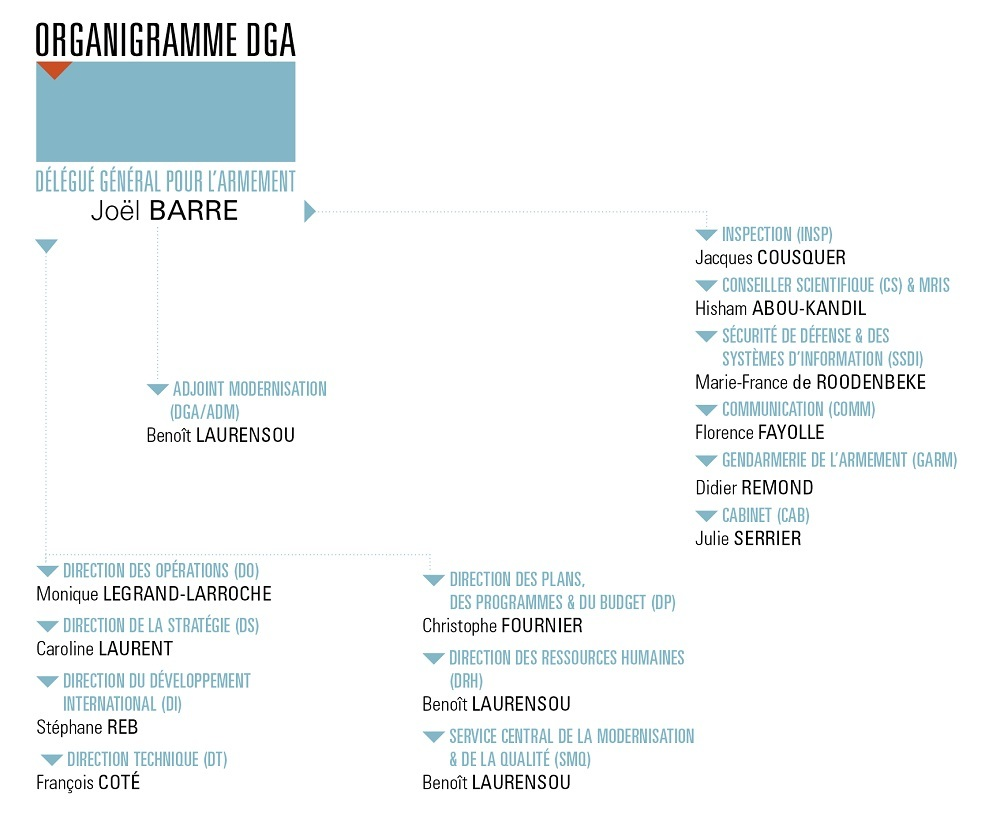
\includegraphics[width=\textwidth]{Organigramme_DGA}
				\caption{Organigramme de la DGA\cite{OrganigrammeDGA}}
				\label{fig:Organigramme_DGA}
			\end{figure}
		\newpage\section{Hiérarchie des Ministères Français à VIM/VSE}\label{sec:hierarchieministereavim}
			\begin{figure}[H]
				\centering
				\resizebox{1.05\textwidth}{!}{\import{figures/}{Hierarchie_Ministeres_a_VIM.tex}}
				\caption{Hiérarchie des Ministères Français à VIM/VSE}
				\label{fig:Hierarchie_Ministeres_a_VIM}
			\end{figure}
		\newpage\section{GUI Qt de GenDbg}\label{sec:guiqtgendbg}
			\begin{figure}[H]
				\hspace*{-1cm}
				\centering
				\fbox{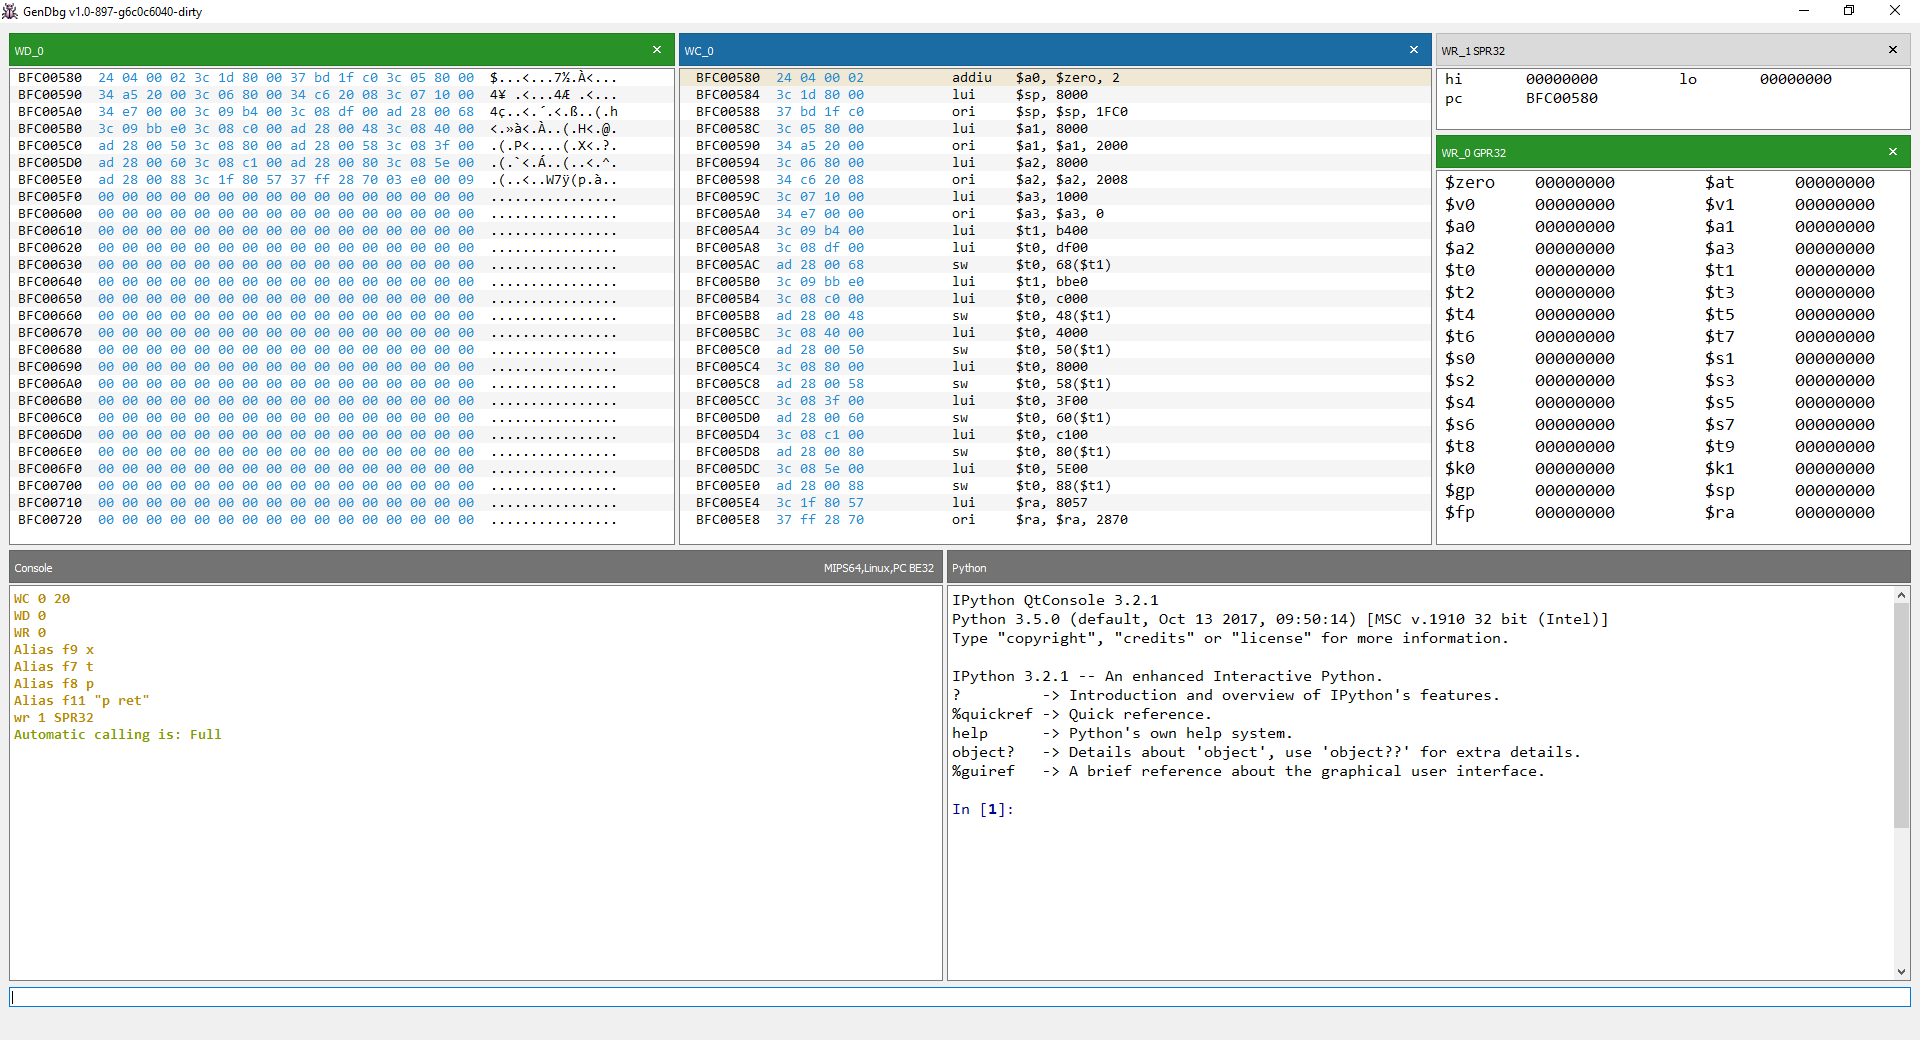
\includegraphics[width=1.1\textwidth]{GenDbg_GUI_Qt}}\\
				%\vspace*{1em}
				%\hspace*{-1cm}
				%\fbox{\resizebox{1.1\textwidth}{!}{\import{figures/}{GenDbg_GUI_Qt_Annotations.tex}}}
				\caption{\acrshort{GUI} Qt de GenDbg}
				\label{fig:GenDbg_GUI_Qt}
			\end{figure}
			\begin{figure}[H]
				\hspace*{-1cm}
				\centering
				\fbox{\resizebox{1.1\textwidth}{!}{\import{figures/}{GenDbg_GUI_Qt_Annotations.tex}}}
				\caption{\acrshort{GUI} Qt de GenDbg: lecture}
				\label{fig:GenDbg_GUI_Qt_Annotations}
			\end{figure}
		\newpage\section{GUI Qt de GenDbg: lecture de la vue code}\label{sec:guiqtgendbgvuecode}
			\begin{figure}[H]
				\hspace*{-1cm}
				\centering
				\resizebox{1.1\textwidth}{!}{\import{figures/}{GenDbg_GUI_Qt_Vue_code_Annotations.tex}}
				\caption{\acrshort{GUI} Qt de GenDbg: lecture de la vue code}
				\label{fig:GenDbg_GUI_Qt_Vue_code_Annotations}
			\end{figure}
\end{document}
